% This is text associated with the open textbook "Open Electromagnetics"
% See immediately below for author, date
% This work is licensed under the Creative Commons Attribution-ShareAlike 4.0 International License. (CC BY-SA 4.0) 
% To view a copy of the license, visit http://creativecommons.org/licenses/by-sa/4.0/

%ORB TITLE Electric Field Due to a Continuous Distribution of Charge
%ORB AUTHOR 0        # S.W. Ellingson, Virginia Tech (ellingson@vt.edu)
%ORB DATE 20180803   # yyyymmdd
%ORB ABSTRACT Electric Field Due to a Continuous Distribution of Charge

\label{m0104_E_due_to_a_Continuous_Distribution_of_Charge} % <-- Must match name of this file and module directory name.  Don't mess with this!

The electric field intensity associated with $N$ charged particles is (Section~\ref{m0103_E_due_to_Point_Charges}):
%
\begin{equation}
{\bf E}({\bf r}) = \frac{1}{4\pi\epsilon} \sum_{n=1}^{N} {   \frac{{\bf r}-{\bf r}_n}{\left|{\bf r}-{\bf r}_n\right|^3}~q_n}
\label{m0104_eCountable}
\end{equation}
%
where $q_n$ and ${\bf r}_n$ are the charge and position of the $n^{\mbox{th}}$ particle.
However, it is common to have a continuous distribution of charge as opposed to a countable number of charged particles.
In this section, we extend Equation~\ref{m0104_eCountable} using the concept of continuous distribution of charge (Section~\ref{m0100_Charge_Distributions}) so that we may address this more general class of problems.

%---------------------------------------------------

{\bf Distribution of Charge Along a Curve.}
\index{charge density!line}
Consider a continuous distribution of charge along a curve $\mathcal{C}$.
The curve can be divided into short segments of length $\Delta l$.  
Then, the charge associated with the $n^{\mbox{th}}$ segment, located at ${\bf r}_n$, is
%
\begin{equation}
q_n = \rho_l({\bf r}_n)~\Delta l
\end{equation}
%
where $\rho_l$ is charge density (units of C/m) at ${\bf r}_n$.
Substituting this expression into Equation~\ref{m0104_eCountable}, we obtain
%
\begin{equation}
{\bf E}({\bf r}) = \frac{1}{4\pi\epsilon} \sum_{n=1}^{N} {   \frac{{\bf r}-{\bf r}_n}{\left|{\bf r}-{\bf r}_n\right|^3}~\rho_l({\bf r}_n)~\Delta l}
\end{equation}
%
Taking the limit as $\Delta l\to 0$ yields:
%
\begin{equation}
\boxed{
{\bf E}({\bf r}) = \frac{1}{4\pi\epsilon} \int_{\mathcal C} {   \frac{{\bf r}-{\bf r}'}{\left|{\bf r}-{\bf r}'\right|^3}~\rho_l({\bf r}')~dl}
}
\label{m0104_eLineCharge}
\end{equation}
%
where ${\bf r}'$ represents the varying position along ${\mathcal C}$ with integration.

The simplest example of a curve is a straight line.
It is straightforward to use Equation~\ref{m0104_eLineCharge} to determine the electric field due to a distribution of charge along a straight line.
However, it is much easier to analyze that particular distribution using Gauss' Law, as shown in Section~\ref{m0149_E_due_to_Inf_Line_Charge}.
The following example addresses a charge distribution for which Equation~\ref{m0104_eLineCharge} is more appropriate.

%ORB EXAMPLE
~\\ \begin{example} 
\begin{mdframed}[backgroundcolor=brown!20,linecolor=brown!20]\raggedright
Electric field along the axis of a ring of uniformly-distributed charge.
\\~\\
Consider a ring of radius $a$ in the $z=0$ plane, centered on the origin, as shown in Figure~\ref{m0104_fRing}.
Let the charge density along this ring be uniform and equal to $\rho_l$ (C/m).
Find the electric field along the $z$ axis.

{\bf Solution.}
The source charge position is given in cylindrical coordinates as
%
\begin{equation}
{\bf r}' = \hat{\bf \rho}a  
\end{equation}
%
The position of a field point along the $z$ axis is simply
%
\begin{equation}
{\bf r} = \hat{\bf z}z  
\end{equation}
%
Thus,
%
\begin{equation}
{\bf r}-{\bf r}' = -\hat{\bf \rho}a + \hat{\bf z}z  
\end{equation}
%
and
%
\begin{equation}
\left|{\bf r}-{\bf r}'\right| = \sqrt{a^2+z^2} 
\end{equation}

Equation~\ref{m0104_eLineCharge} becomes:
%
\begin{equation}
{\bf E}(z) = \frac{1}{4\pi\epsilon} \int_{0}^{2\pi} { \frac{-\hat{\bf \rho}a + \hat{\bf z}z}{\left[a^2+z^2\right]^{3/2}}~\rho_l~\left(a~d\phi\right)}
\end{equation}
%
Pulling factors that do not vary with $\phi$ out of the integral and factoring into separate integrals for the $\hat{\bf \phi}$ and $\hat{\bf z}$ components, we obtain:
%
\begin{equation}
\frac{\rho_l~a}{4\pi\epsilon\left[a^2+z^2\right]^{3/2}} \left[ -a\int_{0}^{2\pi}{\hat{\bf \rho}~d\phi} 
                                                               +\hat{\bf z}z\int_{0}^{2\pi} {d\phi}  \right] 
\end{equation}
%
The second integral is equal to $2\pi$.
The first integral is equal to zero.
To see this, note that the integral is simply summing values of $\hat{\bf\rho}$ for all possible values of $\phi$.  
Since $\hat{\bf\rho}(\phi+\pi)=-\hat{\bf\rho}(\phi)$, the integrand for any given value of $\phi$ is equal and opposite the integrand $\pi$ radians later.
(This is one example of a \emph{symmetry} argument.)  
Thus, we obtain
%
\begin{equation}
{\bf E}(z) = \hat{\bf z}\frac{\rho_l~a}{2\epsilon}\frac{z}{\left[a^2+z^2\right]^{3/2}} 
\end{equation}
%
It is a good exercise to confirm that this result is dimensionally correct.
% *** TODO Above as a problem. 
It is also recommended to confirm that when $z\gg a$, the result is approximately the same as that expected from a particle having the same total charge as the ring.
% *** TODO Above as a problem.
\end{mdframed}
%
\begin{figure}
\begin{center}
\pdftooltip{{  % note double braces
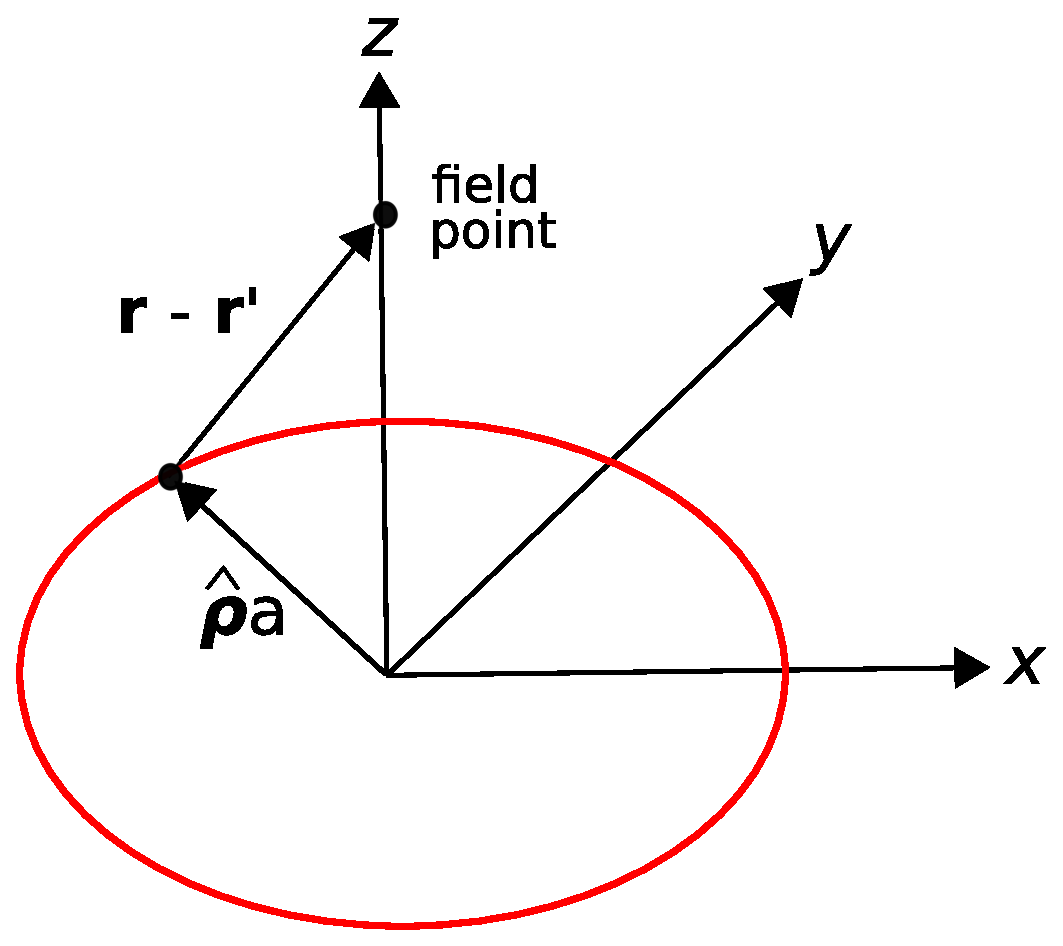
\includegraphics[width=2.5in]{modules/m0104_fRing.eps}
% https://commons.wikimedia.org/wiki/File:M0104_fRing.svg
}}{Cartesian coorinate system shown with x, y, and z axes. A red ring lies in the x and y plane, with its center at the origin. The radius of the circle is labeled bold rho hat * a. From the point at which the radius reaches the outside of the circle extends a ray labeled bold r - bold r', pointing to an arbitrary field point along the z-axis. }
\end{center} 
\centerline{\scriptsize 
\copyright~\hyperref[m0104_fRing_Credit]{K.\ Kikkeri} 
\href{https://creativecommons.org/licenses/by-sa/4.0/}{CC BY~SA 4.0} 
} 
\caption{
\label{m0104_fRing}
Calculating the electric field along the axis of a ring of charge.
}
\end{figure}
\end{example}

%---------------------------------------------------

{\bf Distribution of Charge Over a Surface.}
\index{charge density!surface}
Consider a continuous distribution of charge over a surface $\mathcal{S}$.
The surface can be divided into small patches having area $\Delta s$.  
Then, the charge associated with the $n^{\mbox{th}}$ patch, located at ${\bf r}_n$, is
%
\begin{equation}
q_n = \rho_s({\bf r}_n)~\Delta s
\end{equation}
%
where $\rho_s$ is the surface charge density (units of C/m$^2$) at ${\bf r}_n$.
Substituting this expression into Equation~\ref{m0104_eCountable}, we obtain
%
\begin{equation}
{\bf E}({\bf r}) = \frac{1}{4\pi\epsilon} \sum_{n=1}^{N} {   \frac{{\bf r}-{\bf r}_n}{\left|{\bf r}-{\bf r}_n\right|^3}~\rho_s({\bf r}_n)~\Delta s}
\end{equation}
%
Taking the limit as $\Delta s\to 0$ yields:
%
\begin{equation}
\boxed{
{\bf E}({\bf r}) = \frac{1}{4\pi\epsilon} \int_{\mathcal S} {   \frac{{\bf r}-{\bf r}'}{\left|{\bf r}-{\bf r}'\right|^3}~\rho_s({\bf r}')~ds}
}
\label{m0104_eSurfCharge}
\end{equation}
%
where ${\bf r}'$ represents the varying position over ${\mathcal S}$ with integration.

%ORB EXAMPLE
~\\ \begin{example} 
\begin{mdframed}[backgroundcolor=brown!20,linecolor=brown!20]\raggedright
Electric field along the axis of a disk of uniformly-distributed charge.
\\~\\
Consider a circular disk of radius $a$ in the $z=0$ plane, centered on the origin, as shown in Figure~\ref{m0104_fDisk}.
Let the charge density over this disk be uniform and equal to $\rho_s$ (C/m$^2$).
Find the electric field along the $z$ axis.

{\bf Solution.}
The source charge position is given in cylindrical coordinates as
%
\begin{equation}
{\bf r}' = \hat{\bf \rho}\rho  
\end{equation}
%
The position of a field point along the $z$ axis is simply
%
\begin{equation}
{\bf r} = \hat{\bf z}z  
\end{equation}
%
Thus,
%
\begin{equation}
{\bf r}-{\bf r}' = -\hat{\bf \rho}\rho + \hat{\bf z}z  
\end{equation}
%
and
%
\begin{equation}
\left|{\bf r}-{\bf r}'\right| = \sqrt{\rho^2+z^2} 
\end{equation}

Equation~\ref{m0104_eSurfCharge} becomes:
%
\begin{equation}
{\bf E}(z) = \frac{1}{4\pi\epsilon} \int_{\rho=0}^{a} \int_{\phi=0}^{2\pi} { \frac{-\hat{\bf \rho}\rho + \hat{\bf z}z}{\left[\rho^2+z^2\right]^{3/2}}~\rho_s~\left(\rho~d\rho~d\phi\right)}
\end{equation}
%
To solve this integral, first rearrange the double integral into a single integral over $\phi$ followed by integration over $\rho$:
%
\begin{equation}
\frac{\rho_s}{4\pi\epsilon} \int_{\rho=0}^{a} { \frac{\rho}{\left[\rho^2+z^2\right]^{3/2}}
                                                \left[
                                                \int_{\phi=0}^{2\pi} {
                                                                      \left(-\hat{\bf \rho}\rho + \hat{\bf z}z \right) d\phi
                                                                     }
                                                \right]
                                                d\rho      
                                              }
\label{m0104_eDisk1}
\end{equation}
%
Now we address the integration over $\phi$ shown in the square brackets in the above expression:
%
\begin{equation}
\int_{\phi=0}^{2\pi} { \left(-\hat{\bf \rho}\rho + \hat{\bf z}z \right) d\phi } 
= -\rho\int_{\phi=0}^{2\pi} { \hat{\bf \rho} d\phi } 
+ \hat{\bf z}z\int_{\phi=0}^{2\pi} { d\phi } 
\end{equation}
%
The first integral on the right is zero for the following reason.
As the integral progresses in $\phi$, the vector $\hat{\bf \rho}$ rotates.  
Because the integration is over a complete revolution (i.e., $\phi$ from 0 to $2\pi$), 
the contribution from each pointing of $\hat{\bf \rho}$ is canceled out by another pointing of $\hat{\bf \rho}$ that is in the opposite direction. 
Since there is an equal number of these canceling pairs of pointings, the result is zero.
Thus:
%
\begin{flalign}
\int_{\phi=0}^{2\pi} { \left(-\hat{\bf \rho}\rho + \hat{\bf z}z \right) d\phi }  &= 0 + \hat{\bf z}z\int_{\phi=0}^{2\pi} { d\phi } \nonumber \\
                                                                                 &= \hat{\bf z}2\pi z
\end{flalign}
%
Substituting this into Expression~\ref{m0104_eDisk1} we obtain:
%
\begin{flalign}
~&
\frac{\rho_s}{4\pi\epsilon} \int_{\rho=0}^{a} { \frac{\rho}{\left[\rho^2+z^2\right]^{3/2}}
                                                \left[
                                                \hat{\bf z}2\pi z
                                                \right]
                                                d\rho      
                                              } \nonumber \\
=& \hat{\bf z}\frac{\rho_s z}{2\epsilon} \int_{\rho=0}^{a} { \frac{\rho~d\rho}{\left[\rho^2+z^2\right]^{3/2}} }
\end{flalign}
%
This integral can be solved using integration by parts and trigonometric substitution. 
Since the solution is tedious and there is no particular principle of electromagnetics demonstrated by this solution, we shall simply state the result:
%
\begin{flalign}
\int_{\rho=0}^{a} { \frac{\rho~d\rho}{\left[\rho^2+z^2\right]^{3/2}} } &= \left.\frac{-1}{\sqrt{\rho^2+z^2}}\right|_{\rho=0}^a \nonumber \\
                                                                       &= \frac{-1}{\sqrt{a^2+z^2}} + \frac{1}{\left|z\right|}
\end{flalign}
%
Substituting this result:
%
\begin{flalign}
{\bf E}(z) &= \hat{\bf z}\frac{\rho_s z}{2\epsilon} \left( \frac{-1}{\sqrt{a^2+z^2}} + \frac{1}{\left|z\right|} \right) \nonumber \\
                 &= \hat{\bf z}\frac{\rho_s  }{2\epsilon} \left( \frac{-z}{\sqrt{a^2+z^2}} + \frac{z}{\left|z\right|} \right) \nonumber \\
                 &= \hat{\bf z}\frac{\rho_s  }{2\epsilon} \left( \frac{-z}{\sqrt{a^2+z^2}} + \mbox{sgn}~z                  \right) 
\end{flalign}
%
where ``sgn'' is the ``signum'' 
\index{signum (sgn) function}
function; i.e., $\mbox{sgn}~z =+1$ for $z>0$ and $\mbox{sgn}~z =-1$ for $z<0$.
Summarizing:
%
\begin{equation}
{\bf E}(z) = \hat{\bf z}\frac{\rho_s  }{2\epsilon} \left( \mbox{sgn}~z - \frac{z}{\sqrt{a^2+z^2}} \right)
\label{m0104_eDisk2}
\end{equation}
%
It is a good exercise to confirm that this result is dimensionally correct and yields an electric field vector that points in the expected direction  and with the expected dependence on $a$ and $z$.
%%% TODO problem to do the above
\end{mdframed}
%
\begin{figure}
\begin{center}
\pdftooltip{{  % note double braces
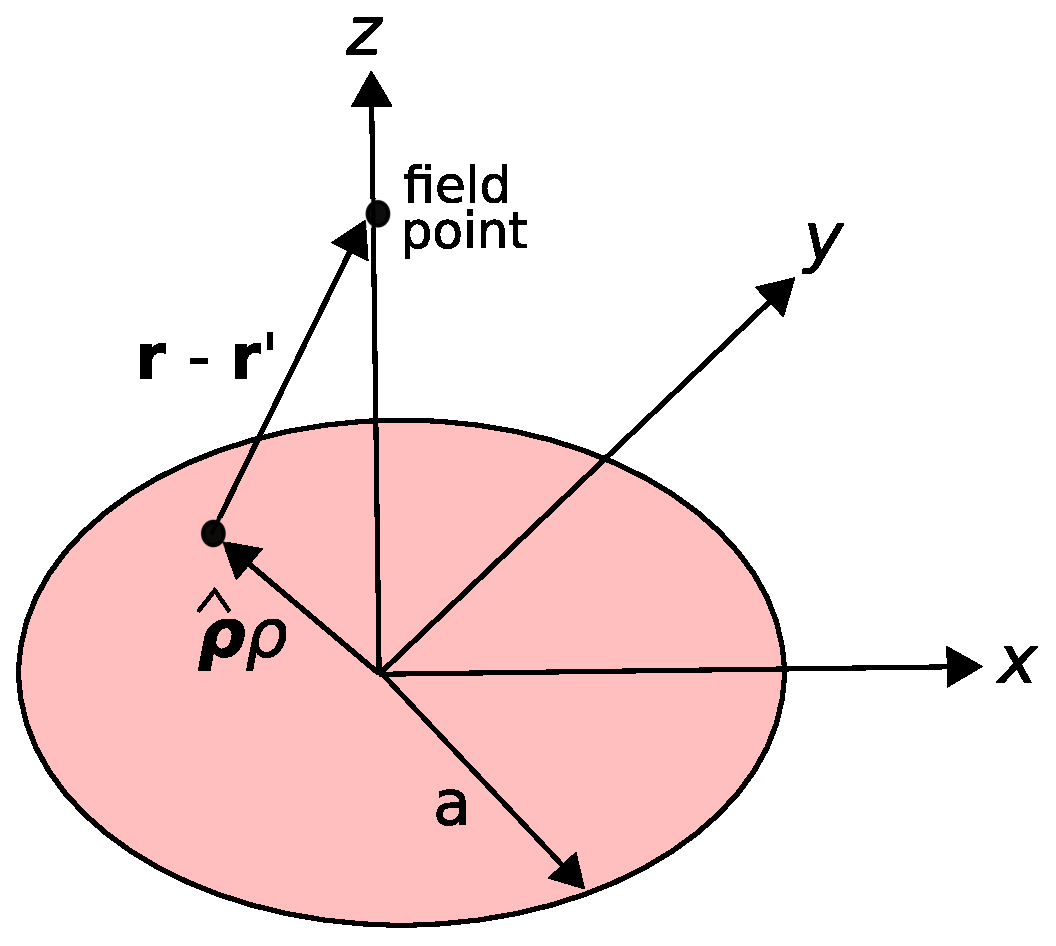
\includegraphics[width=2.5in]{modules/m0104_fDisk.eps}
% https://commons.wikimedia.org/wiki/File:M0104_fDisk.svg
}}{Cartesian coordinate system with x, y, and z axes. A red disk lies in the x-y plane, with its center at the origin and a radius (a). A ray labeled bold rho hat * rho points toward an arbitrary point in the disk. From that point, a ray labeled bold r - bold r superscript 1 points toward an arbitrary field point on the z-axis. }
\end{center} 
\centerline{\scriptsize 
\copyright~\hyperref[m0104_fDisk_Credit]{K.\ Kikkeri} 
\href{https://creativecommons.org/licenses/by-sa/4.0/}{CC BY~SA 4.0} 
} 
\caption{
\label{m0104_fDisk}
Calculating the electric field along the axis of a disk of charge.
}
\end{figure}
\end{example}


A special case of the ``disk of charge'' scenario considered in the preceding example is an \emph{infinite sheet} of charge.
The electric field from an infinite sheet of charge is a useful theoretical result.  
We get the field in this case simply by letting $a\to\infty$ in Equation~\ref{m0104_eDisk2}, yielding:
%
\begin{equation}
{\bf E}({\bf r}) = \hat{\bf z}\frac{\rho_s}{2\epsilon} \mbox{sgn}~z
\label{m0104_eISC}
\end{equation}
%
Again, it is useful to confirm that this is dimensionally correct: C/m$^2$ divided by F/m yields V/m.
Also, note that Equation~\ref{m0104_eISC} is the electric field at \emph{any} point above or below the charge sheet -- not just on $z$ axis.  This follows from symmetry.  From the perspective of any point in space, the edges of the sheet are the same distance (i.e., infinitely far) away.

%---------------------------------------------------

{\bf Distribution of Charge In a Volume.}
\index{charge density!volume}
Consider a continuous distribution of charge within a volume $\mathcal{V}$.
The volume can be divided into small cells (volume elements) having volume $\Delta v$.  
Then, the charge associated with the $n^{\mbox{th}}$ cell, located at ${\bf r}_n$, is
%
\begin{equation}
q_n = \rho_v({\bf r}_n)~\Delta v
\end{equation}
%
where $\rho_v$ is volume charge density (units of C/m$^3$) at ${\bf r}_n$.
Substituting this expression into Equation~\ref{m0104_eCountable}, we obtain
%
\begin{equation}
{\bf E}({\bf r}) = \frac{1}{4\pi\epsilon} \sum_{n=1}^{N} {   \frac{{\bf r}-{\bf r}_n}{\left|{\bf r}-{\bf r}_n\right|^3}~\rho_v({\bf r}_n)~\Delta v}
\end{equation}
%
Taking the limit as $\Delta v\to 0$ yields:
%
\begin{equation}
\boxed{
{\bf E}({\bf r}) = \frac{1}{4\pi\epsilon} \int_{\mathcal V} {   \frac{{\bf r}-{\bf r}'}{\left|{\bf r}-{\bf r}'\right|^3}~\rho_v({\bf r}')~dv}
}
\end{equation}
%
where ${\bf r}'$ represents the varying position over ${\mathcal V}$ with integration.

% %ORB EXAMPLE
% ~\\ \begin{example} 
% \begin{mdframed}[backgroundcolor=green!20] 
% Electric Field Due to a Uniform Distribution of Charge over a Cube
% \end{mdframed}
% {\color{red}NEED TO COMPLETE.}
% \centerline{\rule{2in}{1pt}} \end{example}





